
\includegraphics[height=1.25cm]{images/pictograms/pic}

\includegraphics[height=1.25cm]{images/pictograms/FEM}
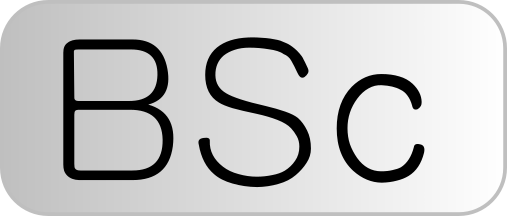
\includegraphics[height=1.25cm]{images/pictograms/bsc}

%%%%%%%%%%%%%%%%%%%%%%%%%%%%%%%%%%%%%%%%%%%%%%%%%%%%%%%%%%%%%%%%%%%%%%%%%%%%%%%%%%%%%%%%%%%%

%\lstinputlisting[language=bash,basicstyle=\small]{python_codes/fieldstone_13/keywords.key}

\begin{center}
\inpython 
{\small Code: \url{https://github.com/cedrict/fieldstone/tree/master/python_codes/fieldstone_13}}
\end{center}

\par\noindent\rule{\textwidth}{0.4pt}

{\sl This fieldstone was developed in collaboration with BSc student Eric Hoogen}. 
\index{contributors}{E. Hoogen}

\par\noindent\rule{\textwidth}{0.4pt}

Last revision: September 26th, 2025.

\par\noindent\rule{\textwidth}{0.4pt}

%%%%%%%%%%%%%%%%%%%%%%%%%%%%%%%%%%%%%%%%%%%%%%%%%%%%%%%%%%%%%%%%%%%%%%%%%%%%%%%%%%%%%%%%%%%%

This \stone deals with the Particle-in-Cell method where 
Lagrangian points are first distributed in the domain and 
subsequently advected with the flow.

After the initial setup of the grid, particles are
generated and placed in the domain. One could simply randomly generate 
the particles position in the whole domain but unless a {\it very} large 
number of particles is used, the chance that an element does 
not contain any particle at all does exists and this will prove problematic. 
In order to get a better control over the particles spatial distribution, 
one usually generates the particles per element, so that the total 
number of particles in the domain is the product of the number of 
elements \lstinline{nel} times the user-chosen initial number of particles 
per element \lstinline{nparticle_per_element}.

Our next concern is how to actually place the particles inside an element. 
Two methods come to mind: on a regular grid, or in a random manner, 
as shown on the following figure:

\begin{center}
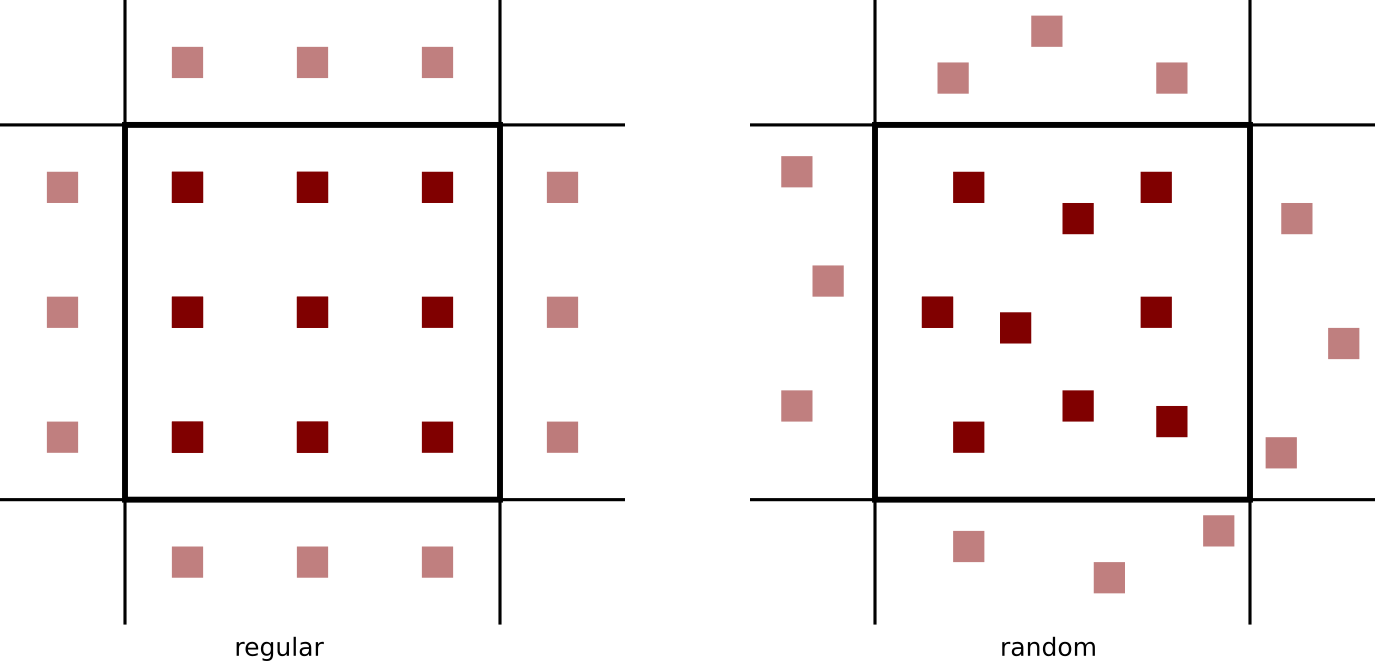
\includegraphics[width=9cm]{python_codes/fieldstone_13/images/markers} 
\end{center}

In both cases we make use of the basis functions: we generate the 
positions of the markers (random or regular) in the reference
element first ($r_{ip},s_{ip}$), and then map those out to the real element as follows:
\begin{equation}
x_{ip}=\sum_k^m \bN_k(r_{ip},s_{ip}) x_k
\quad\quad\quad\quad
y_{ip}=\sum_k^m \bN_k(r_{ip},s_{ip}) y_k
\end{equation}
where $x_k,y_k$ are the coordinates of the vertices/nodes of the element.

A third option consists in the use of the so-called Poisson-disc sampling which 
produces points that are tightly-packed, but no closer to each other than 
a specified minimum distance, resulting in a more natural pattern 
\footnote{https://en.wikipedia.org/wiki/Supersampling}. Note that 
1) the Poisson-disc algorithm fills the whole domain at once, not element after element;
2) the code used to generate this distribution is taken from 
\url{https://scipython.com/blog/poisson-disc-sampling-in-python/}.

{\color{red} say smthg about avrg dist}  

\begin{center}
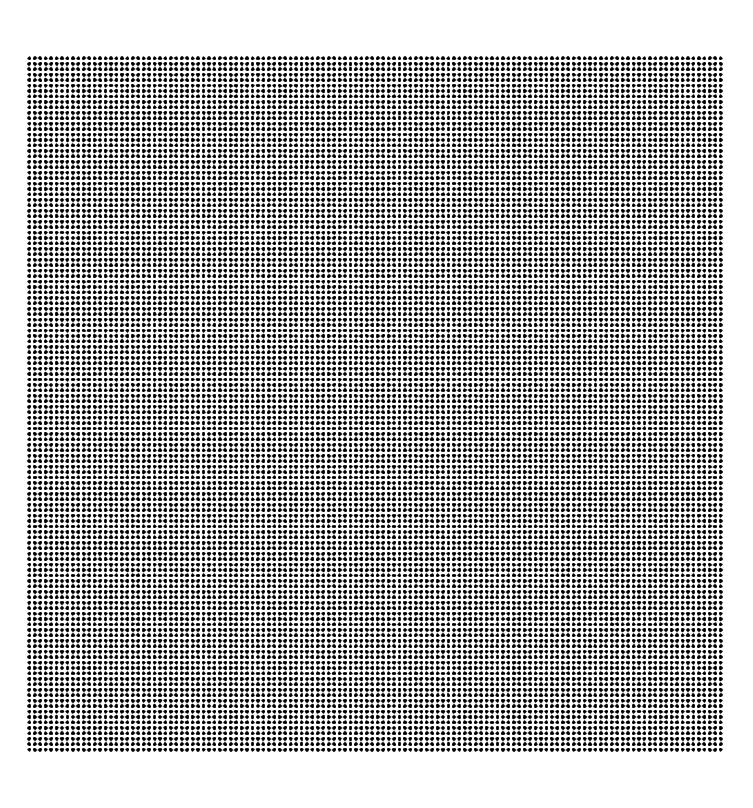
\includegraphics[width=5.7cm]{python_codes/fieldstone_13/images/markers_reg} 
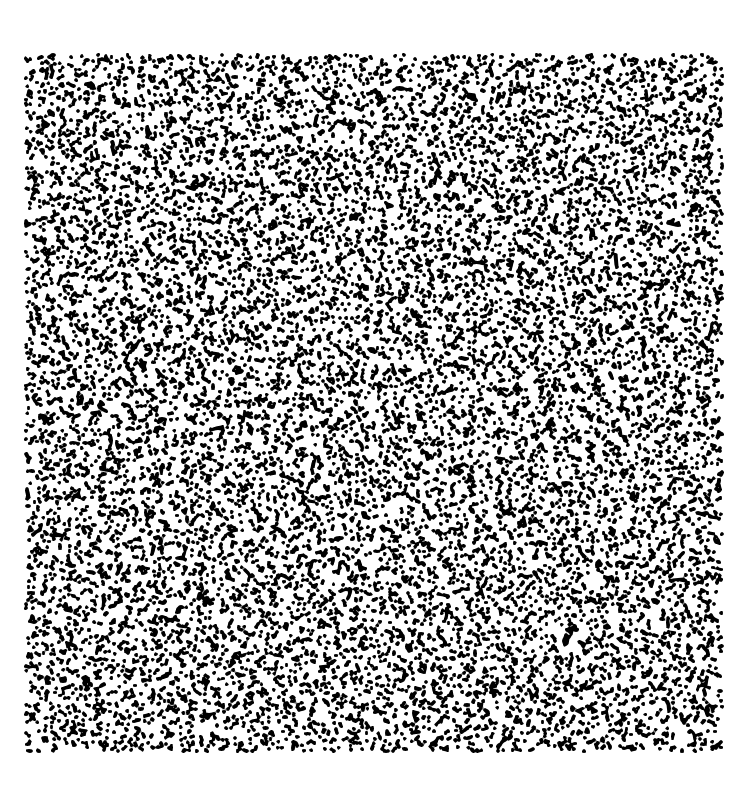
\includegraphics[width=5.7cm]{python_codes/fieldstone_13/images/markers_rand} 
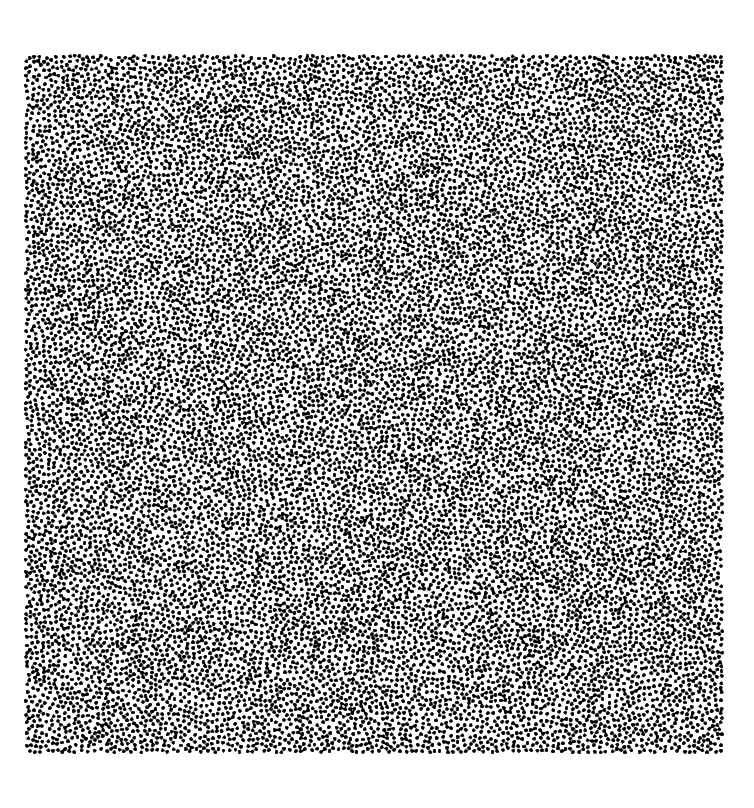
\includegraphics[width=5.7cm]{python_codes/fieldstone_13/images/markers_pd} \\
{\captionfont Left: regular distribution, middle: random, right: Poisson disc.\\
 16384 markers ($32 \times 32$ grid, 16 markers per element).}
\end{center}


When using {\it active} particles (i.e. their properties are projected 
back onto the FE mesh and used to compute coefficients of the PDEs), 
one is faced with the problem of transferring the properties they carry to 
the mesh on which the PDEs are to be solved. 

As we have seen, building the FE matrix involves a loop over all elements, 
so one simple approach consists of assigning each element a single property
computed as the average of the values carried by the markers in that element. 
Often in colloquial language ``average'' refers to the arithmetic mean: 
\begin{equation}
\langle \phi \rangle_{am}=\frac{1}{n} \sum_{ip=1}^n \phi_{ip} 
\end{equation}
where $<\phi>_{am}$ is the arithmetic average of the $n$ numbers $\phi_{ip}$. 
However, in mathematics other means are commonly used, such as the geometric mean: 
\begin{equation}
\langle \phi \rangle_{gm}=\left( \prod_{ip=1}^n \phi_{ip} \right)^{1/n}
\qquad
\text{or}
\qquad
\log \langle \phi \rangle_{gm}= \frac{1}{n} \left( \sum_{ip=1}^n \log \phi_{ip} \right)
\end{equation}
and the harmonic mean
\begin{equation}
\langle \phi \rangle_{hm}=\left( \frac{1}{n} \sum_{ip=1}^n \frac{1}{\phi_{ip}} \right)^{-1}
\end{equation}
Furthermore, there is a well known inequality for any set of positive numbers\footnote{Source?},
\begin{equation}
\langle \phi \rangle_{am}\quad  \geq \quad
\langle \phi \rangle_{gm}\quad  \geq \quad
\langle \phi \rangle_{hm} 
\end{equation}
which will prove to be important later on. 

Let us now turn to a simple concrete example: the 2D Stokes sphere. 
There are two materials in the domain, so that particles carry the label ``mat=1'' or ``mat=2''.
For each element an average density and viscosity need to be computed. 
The majority of elements contains particles
with a single material label so that the choice of averaging does not matter (it is trivial to verify that 
if $\phi_i=\phi_0$ then $\langle \phi \rangle_{am}=\langle \phi \rangle_{gm}=\langle \phi \rangle_{hm}=\phi_0$.
Remain the elements crossed by the interface between the two materials: they contain particles of both materials
and the average density and viscosity inside those depends on 1) the total number of particles inside the element, 
2) the ratio of particles 1 to particles 2, 3) the type of averaging. 

This averaging problem has been studied and documented in the literature, see
for example 
\textcite{scbe08} (2008), \textcite{deka08} (2008), \textcite{thmk14} (2014), 
\textcite{pukp17} (2017).

Let us now turn to the projection of the particle field onto the nodes of the mesh.

\begin{center}
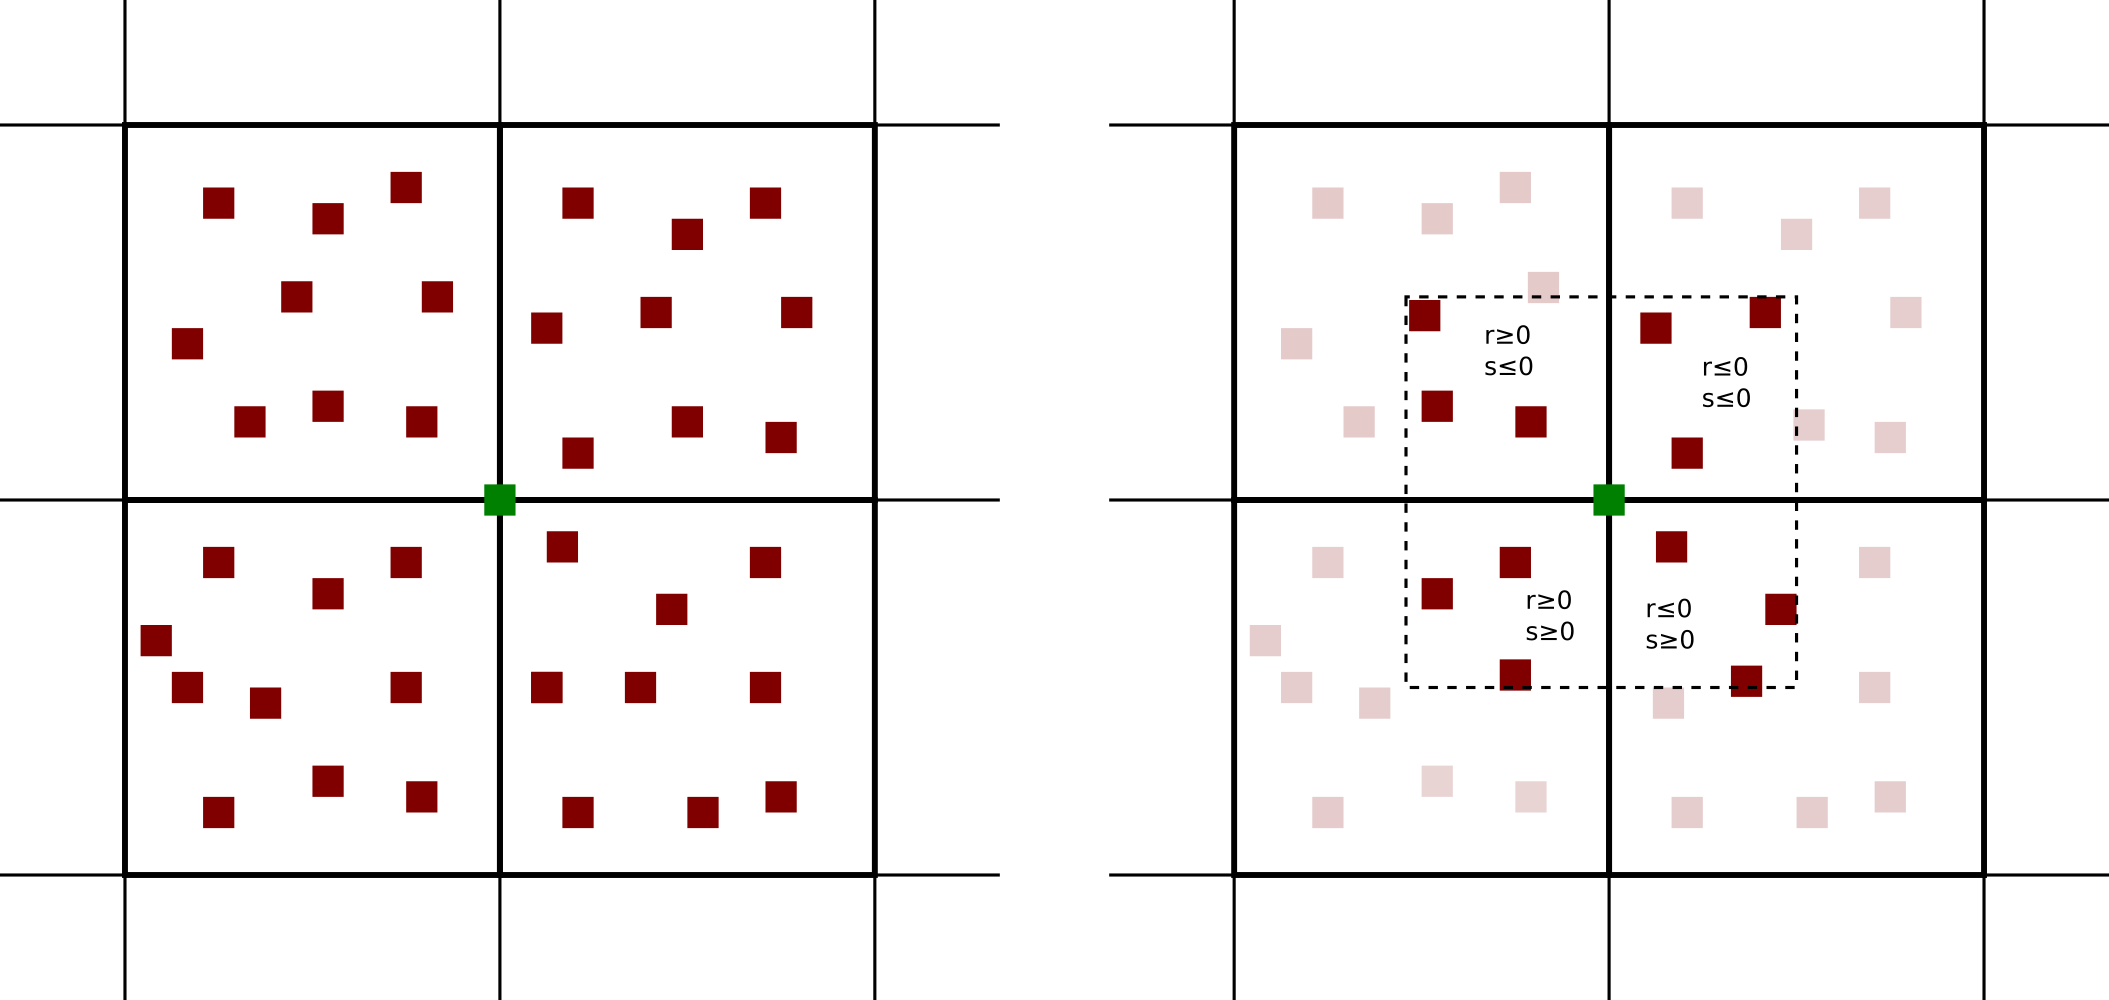
\includegraphics[width=13cm]{python_codes/fieldstone_13/images/markers2}\\
{\captionfont Nodal projection. 
Left: all red particles inside elements to which the green node belongs to are taken into account.
This is the basis for proj=1 algorithm.\\
Right: only the particles closest to the green node count. This is the basis for the proj=2
algorithm.}
\end{center}

Let $k$ be the green node of the figures above. Let $(r,s)$ 
denote the coordinates of a marker inside its element.
For clarity, we define the follow three nodal averaging schemes:
\begin{itemize}
\item nodal type 1: 
\[
f_k = \frac{\text{sum of values carried by markers in 4 neighbour elements}}
{\text{number of markers in 4 neighbour elements}}
\]
\item nodal type 2: 
\[
f_k = \frac{\text{sum of values carried by markers inside dashed line}}
{\text{number of markers in area delimited by the dashed line}}
\]
\item nodal type 3: 
\[
f_k = \frac{\text{sum of values carried by markers in 4 neighbour elements } * \bN^{Q_1}(r,s)}
{\text{sum of }\bN^{Q_1}(r,s)} 
\]
where $\bN^{Q_1}$ is the $Q_1$ basis function corresponding to node $k$ 
defined on each element. Since these 
functions are 1 on node $k$ and then linearly decrease and become zero on 
the neighbouring nodes, this
effectively gives more weight to those markers closest to node $k$.
One could use $Q_2$ or higher order basis functions but it is important 
to remember that those are negative on a part of the reference element
and this could/will pose problems so we rather use positive and monotonously 
decreasing functions instead.
\end{itemize}

The third strategy is adopted in \textcite{mabl14} (2014) and \textcite{mabl15} (2015) 
(although it is used to interpolate onto the nodes of $Q_2 \times P_{-1}$ elements). 
It is formulated as follows:

\begin{displayquote}
{\color{darkgray}
We assume that an arbitrary material point property $f$, is discretized via 
$f(\bm x)\simeq \delta(\bm x - \bm x_p) f_p$. We then utilize an approximate local $L_2$ projection
of $f_p$ onto a continuous $Q_1$ finite element space. The corner vertices of
each $Q_2$ finite element define the mesh $f_p$ is projected onto.
The local reconstruction for a node i is defined by
\[
\hat{f}_i = \frac{\int_{\Omega_i}N_i(\bm x) f(\bm x)}{\int_{\Omega_i} N_i(\bm x)} \simeq
\frac{\sum_p N_i(\bm x_p) f_p }{\sum_p N_i(\bm x_p)}
\]
where the summation over $p$ includes all material points 
contained within the support $\Omega_i$ of the trilinear interpolant $N_i$.}
\end{displayquote}


%---------------------------------------------------------------
\subsection*{Numerical setup}

The setup is a Stokes sphere experiment with radius $R=0.123$ placed in the center 
of the domain which is a $1\times 1$ square. 
The viscosity of the sphere is set to $10^3$ while the viscosity of the 
surrounding fluid is 1. The average density is always computed with an arithmetic mean. 

The code relies on $Q_1 \times P_0$ elements with a penalty formulation for simplicity.
and the penalty parameter is set to $\lambda=10^7$.
No-slip boundary conditions are applied on all four sides.

The bash script {\sl script\_runall} 
runs the code for many resolutions, all three initial particle distributions and all four 
averaging types (elemental, nodal 1,2,3). 

The script loops over the number of markers per dimension (3,4,5,6...), 
the type of projection
(0: elemental, 1: use all four elements around node, 2: use all four quadrants around node
3: use all four elements around node with weighing) and also the type of averaging 
(avrg=1: arithmetic mean; avrg=2: geometric mean; avrg=3: harmonic mean).

The root mean square velocity is used as a proxy for the flow in the domain. 
All results are shown on the next page. 

%---------------------------------------------------------------
\subsection*{Conclusions}

\begin{itemize}
\item
With increasing resolution ($h\rightarrow 0$) $\upnu_{rms}$ 
values seem to converge towards a single value, irrespective 
of the number of markers. 

\item
At low resolution, say $32\times 32$ (i.e. h=0.03125), $\upnu_{rms}$ 
values for the three averagings differ by about 10\%. 
At higher resolution, say $128\times 128$, $\upnu_{rms}$ 
values are still not converged.  

\item
The number of markers per element plays a role at low resolution, 
but less and less with increasing resolution. 

\item
Results for random and regular marker distributions are not 
identical but follow a similar trend and seem to converge to 
the same value.

\item  elemental values yield better results (especially at low resolutions)

\item harmonic mean yields overal the best results

\item the same exercise could/should be repeated with $Q_2\times Q_1$ elements.
\end{itemize}

\newpage
Root mean square velocity results are shown hereunder:
\begin{center}
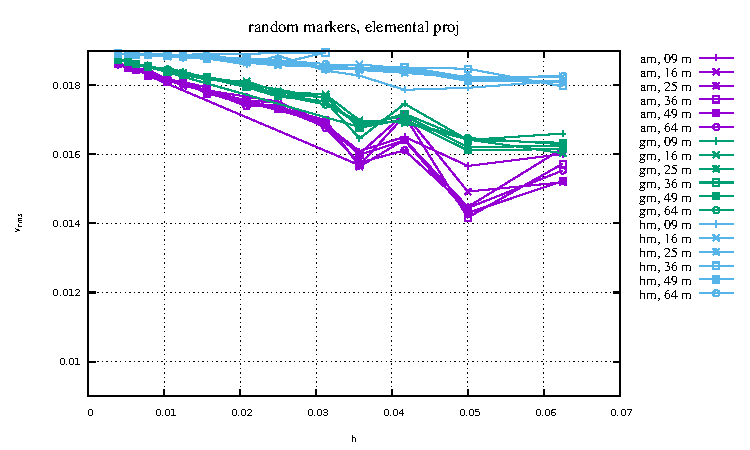
\includegraphics[width=5.7cm]{python_codes/fieldstone_13/RESULTS/vrms_rand_proj0} 
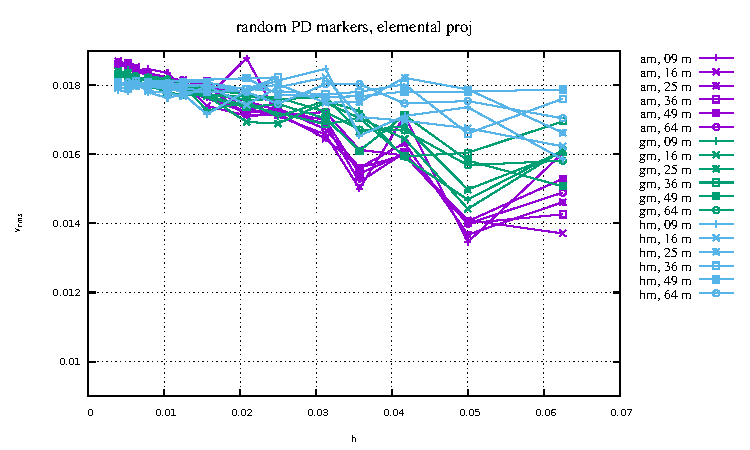
\includegraphics[width=5.7cm]{python_codes/fieldstone_13/RESULTS/vrms_poissondisc_proj0} 
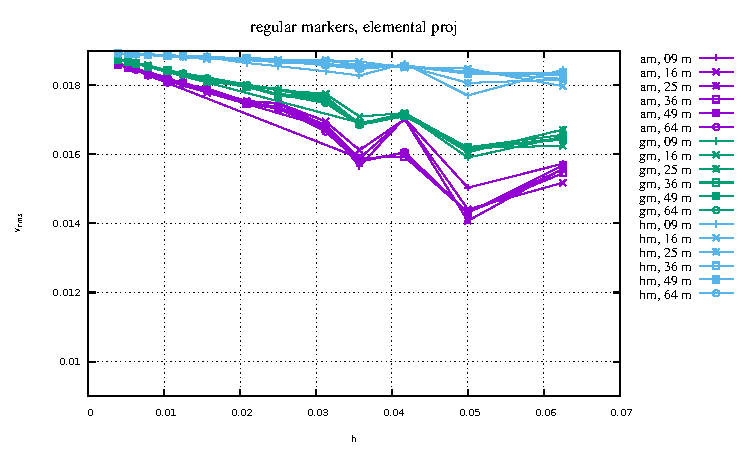
\includegraphics[width=5.7cm]{python_codes/fieldstone_13/RESULTS/vrms_reg_proj0}\\
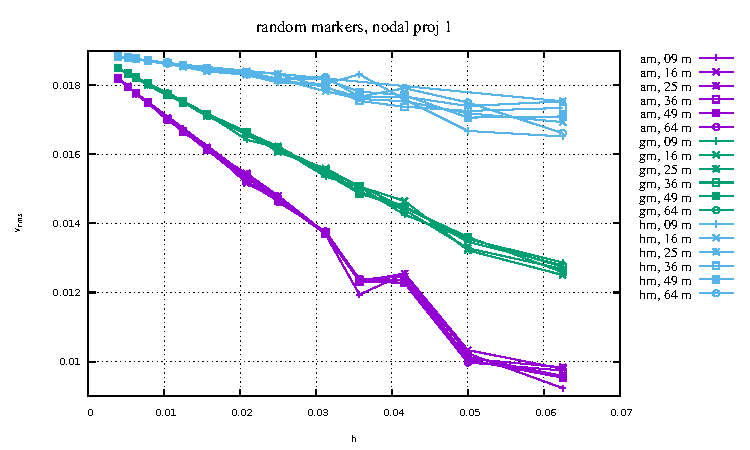
\includegraphics[width=5.7cm]{python_codes/fieldstone_13/RESULTS/vrms_rand_proj1} 
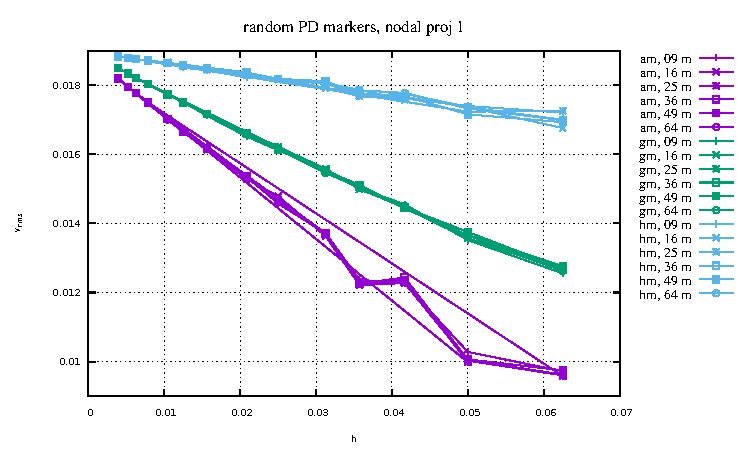
\includegraphics[width=5.7cm]{python_codes/fieldstone_13/RESULTS/vrms_poissondisc_proj1} 
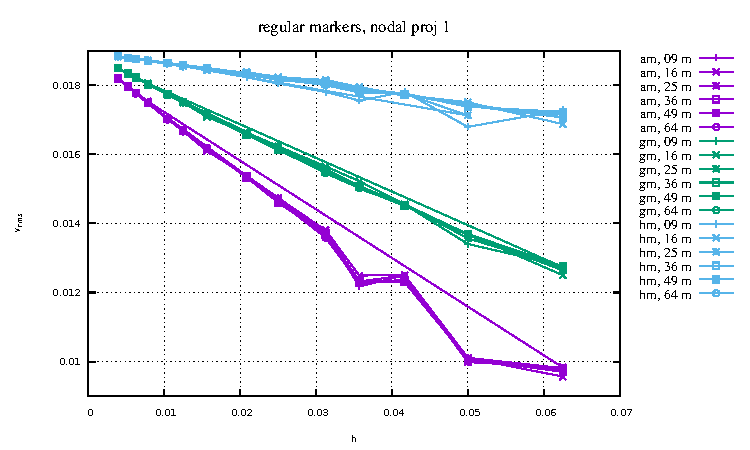
\includegraphics[width=5.7cm]{python_codes/fieldstone_13/RESULTS/vrms_reg_proj1}\\ 
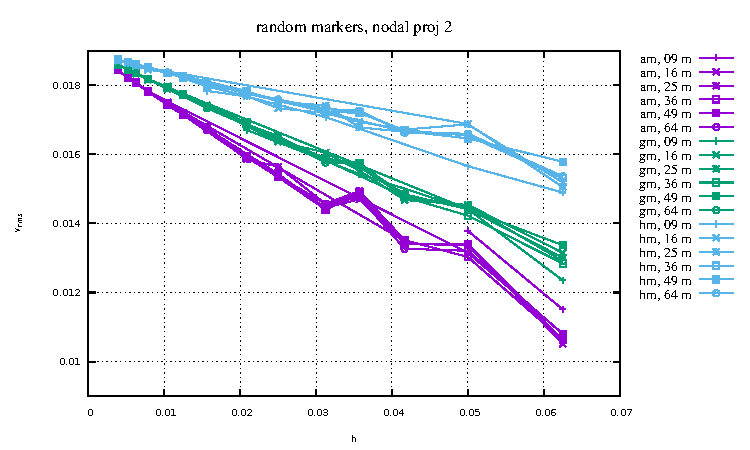
\includegraphics[width=5.7cm]{python_codes/fieldstone_13/RESULTS/vrms_rand_proj2} 
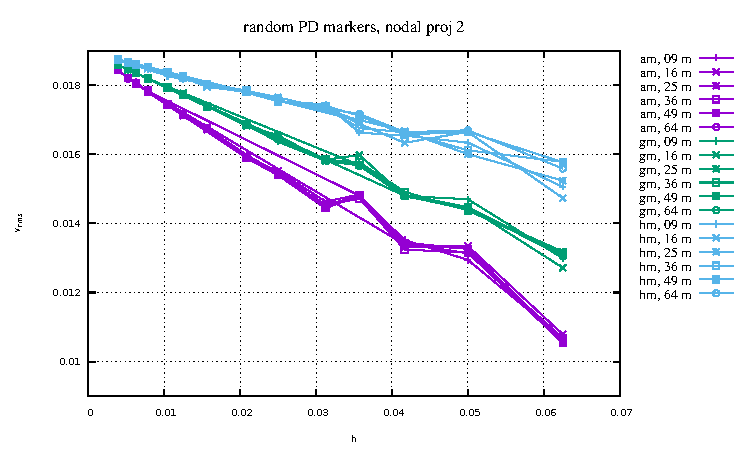
\includegraphics[width=5.7cm]{python_codes/fieldstone_13/RESULTS/vrms_poissondisc_proj2} 
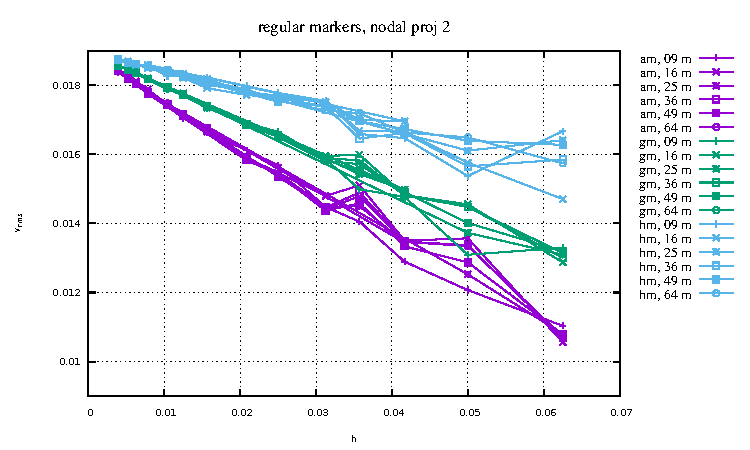
\includegraphics[width=5.7cm]{python_codes/fieldstone_13/RESULTS/vrms_reg_proj2}\\ 
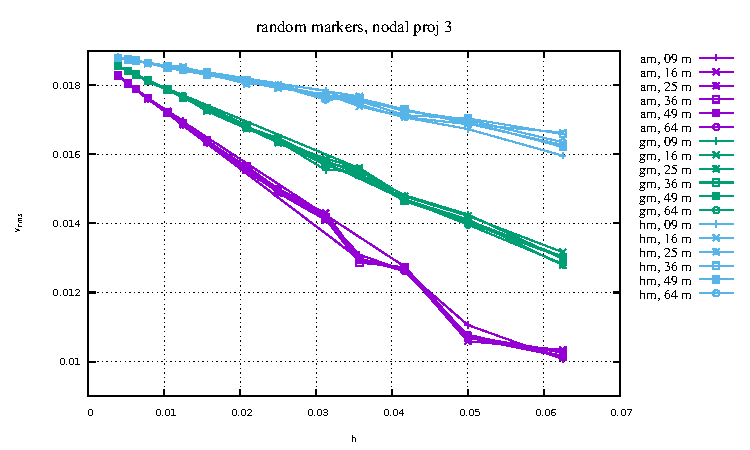
\includegraphics[width=5.7cm]{python_codes/fieldstone_13/RESULTS/vrms_rand_proj3} 
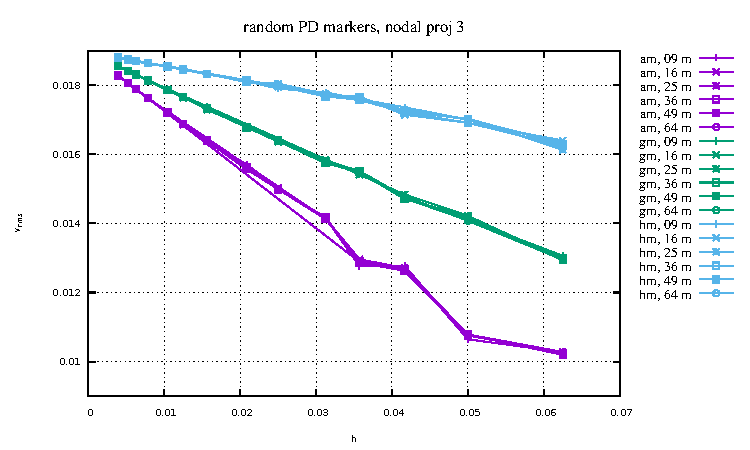
\includegraphics[width=5.7cm]{python_codes/fieldstone_13/RESULTS/vrms_poissondisc_proj3} 
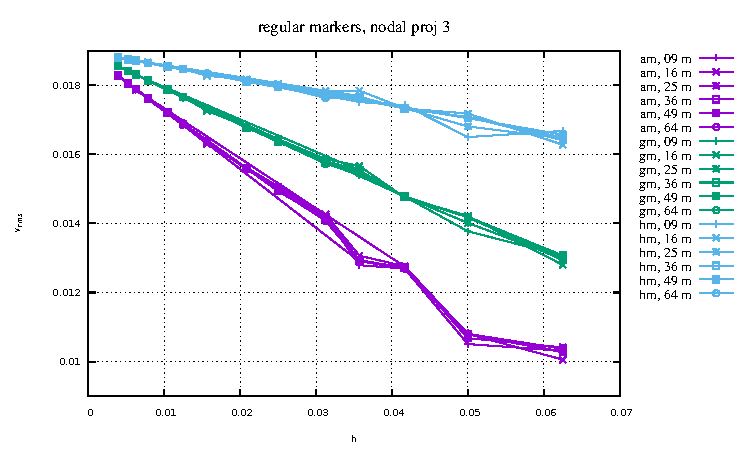
\includegraphics[width=5.7cm]{python_codes/fieldstone_13/RESULTS/vrms_reg_proj3}\\
{\captionfont Left column: random markers, middle column: Poisson disc, 
right column: regular markers. \\
First row: elemental projection, second row: nodal 1 projection, 
third row: nodal 2 projection, fourth row: nodal 3 projection. }
\end{center}

\begin{center}
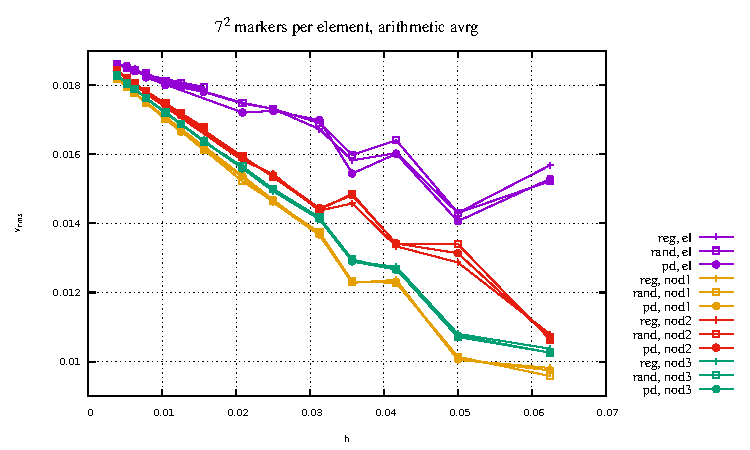
\includegraphics[width=5.7cm]{python_codes/fieldstone_13/RESULTS/vrms_am} 
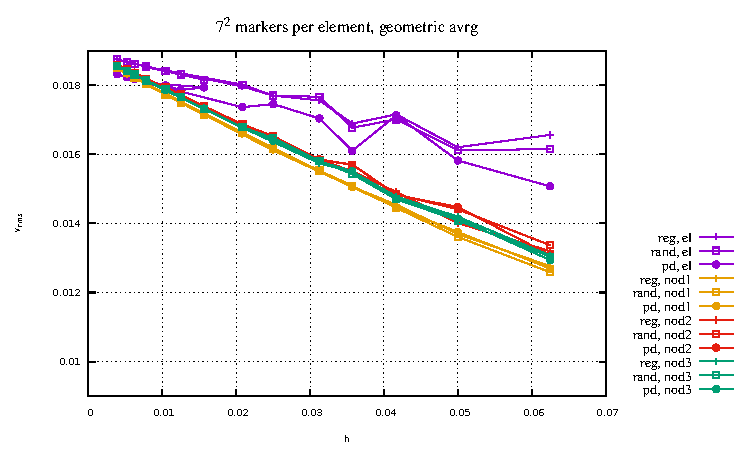
\includegraphics[width=5.7cm]{python_codes/fieldstone_13/RESULTS/vrms_gm} 
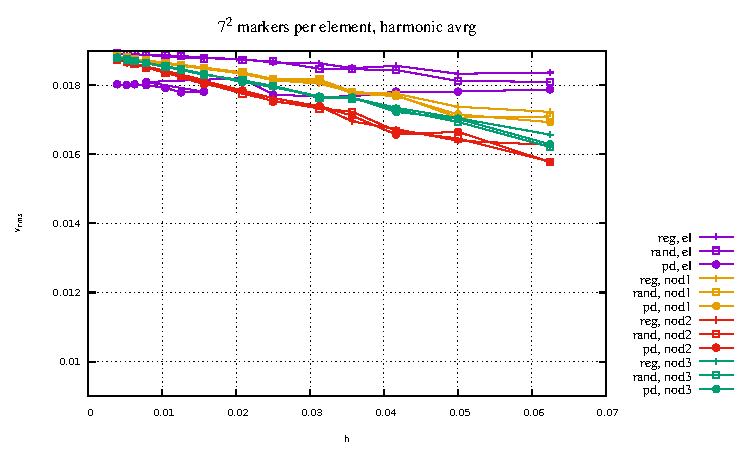
\includegraphics[width=5.7cm]{python_codes/fieldstone_13/RESULTS/vrms_hm}\\
{\captionfont Left to right: arithmetic, geometric, harmonic averaging for viscosity.}
\end{center}

